\chapter{Background}
\section{Machine Learning} \label{Machine Learning}
    As described in the book Deep Learning\cite{Goodfellow-et-al-2016_ML} machine learning can intuitively be split into four parts; The algorithm, empirical data, a task and a performance measure. A machine learning algorithm can then be identified as an algorithm that increases its performance on a task, given data. As this happens, the algorithm is said to be learning. The task itself and the data the algorithm is given may vary. This is why we can approximately divide the machine learning approaches into three categories\cite{Goodfellow-et-al-2016_E}: supervised learning, unsupervised and reinforcement learning. 
    
    \subsection{Algorithm types} \label{Algorithm types}
        \subsubsection{Supervised learning}
            Supervised learning \cite{Goodfellow-et-al-2016_E} algorithms base themselves on datasets containing samples that also have a label. This means the output the algorithm will have to predict. These labels can for example be binary class or consist of a multitude of classes or values in regression problems.
            
        \subsubsection{Unsupervised learning}
            Unlike supervised leaning, the unsupervised learning \cite{Goodfellow-et-al-2016_E} algorithms only have the data and will learn properties contained in the data. A practical example is clustering, where you can divide a dataset into clusters based on similar features. 
                
        \subsubsection{Reinforcement learning}
            In reinforcement learning \cite{Goodfellow-et-al-2016_E}, the algorithm do not learn from a given dataset, but will act in an environment. In some cases this is a feedback loop giving either a positive or negative reward for performing certain actions. The goal is then for the algorithm to maximize this reward. This is what people often associate with \gls{ai} and can be for example seen in the AlphaZero software that beat professional chess players\cite{silver2017mastering}.
    
    \subsection{Data}
        things
    \subsection{Features}
        things
    \subsection{Overfitting vs. underfitting}
        things
    \subsection{Bias - variance tradeoff}
        things
    \subsection{Model evaluation}
        things
    \subsubsection{Train-Val-Test split}
        things
    \subsubsection{Hyperparameter-search}
        things

\section{Artificial Neural Networks} \label{neural networks}
    \citeauthor{Goodfellow-et-al-2016_NN} \cite{Goodfellow-et-al-2016_NN} describes \gls{ann} as a unknown function \textit{\^{f}} that maps an input \textit{x} to an output \textit{y}. The goal is then to approximate some optimal function \textit{f} through learning from examples. In this section, I will explain the basics of \gls{ann}s.

    \subsection{Perceptron} \label{perceptron}
        The \gls{ann}s fundamental building block is called an artificial neuron or perceptron. It is formulated in the following way\cite{razavi2021deep_exp_per}:
            \begin{equation} \label{eq_perceptron}
                y = \sigma(\sum_{i=1}^{D}w_ix_i + b)
            \end{equation}
            
        where D is the number dimension of the input space, x is the input vector and w is a set of weights that is of the same size as x, b is the bias and {\textsigma} is a nonlinear activation function which will be explained later in \ref{activation function}. In short the equation inside the activation functions is a linear regression. The perceptron is illustrated in figure \ref{Perceptron / MLP}.
    
    \subsection{Multi-layered perceptron} \label{MLP}
        The neurons presented in section \ref{perceptron} are then piled together in layers to form a \gls{ann}, which in turn forms what is called a \gls{mlp}.All the neurons in each layer are connected to every neuron in the next layer, as depicted in figure \ref{Perceptron / MLP}.
        
            \begin{figure}[H]
                \centering
                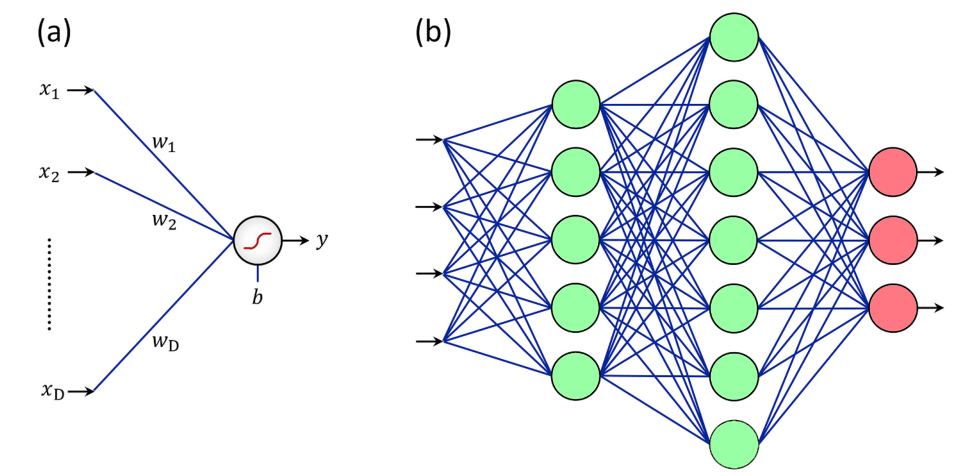
\includegraphics[scale=0.5]{figures/perceptron.png}
                \caption{(a) A perceptron and (b) a multi-layer perceptron with four inputs in the input-layer, two hidden layers(green), and three outputs in the output-layer(red).}
              	\medskip 
            	\hspace*{15pt}\hbox{\scriptsize Credit: Deep learning, explained: Fundamentals, explainability, and bridgeability
        to process-based modelling\cite{razavi2021deep_exp_DL}}
                \label{Perceptron / MLP}
            \end{figure}
        
        The architecture of the \gls{ann} consist of an input layer, a user defined number of hidden layers and finally an output layer. A \gls{mlp} is a type of network called feed-forward \gls{ann} because the data flows from the input to the output layer. The parameters that are adjusted through training (explained in section XXX) are all the weights and biases between every neuron in the network. The intuition for the MLP depicted in \ref{Perceptron / MLP} is that different neurons will fire with varying strengths depending on the input, resulting in different outputs.
        
    \subsection{Activation function} \label{activation function}
        The activations function is what enables the \gls{ann} to learn non-linear features \cite{razavi2021deep_exp_per}. The reason you need it is that a network consisting of only linear layers will just be the same as a single linear layer \cite{razavi2021deep_exp_per}. The activation function used in this thesis was the ReLU which stands for rectified as described in \cite{sharma2019new_activation_func}. The formula for it is as follows:
            \begin{equation} \label{relu_eq}
                f(x) = max(0,x)
            \end{equation}
        As can be seen in figure \ref{activation_fig} the function is 0 while x < 0 and then linear. Intuitively, this function can make a selection of neurons in figure \ref{MLP} send their computed value forth, and some  other neurons output nothing. This can result in greater efficiency and faster training, as not all neurons are active \cite{sharma2019new_activation_func}.
        
        An example of another activation function is the sigmoid \cite{sharma2019new_activation_func}, which transforms the values in the range 0 to 1. I will list the formula and have included it in the plot \ref{activation_fig}, but will not go any further as it is not necessary for understanding this thesis. Sigmoid formula:
            \begin{equation} \label{sigmoid_eq}
                f(x) = \dfrac{1}{e^{-x}} 
            \end{equation}
            
            \begin{figure}[H]
                \centering
                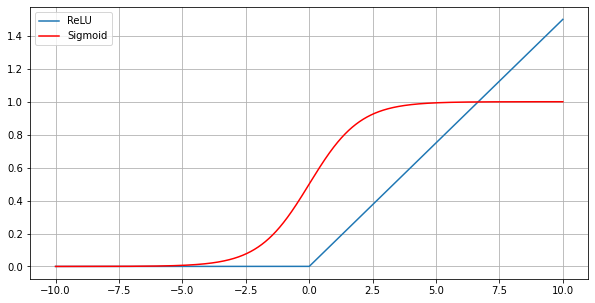
\includegraphics[scale=0.5]{figures/activation.png}
                \caption{A ReLU function (blue) and a sigmoid function (red)}.
              	\medskip 
                \label{activation_fig}
            \end{figure}

\section{Training Neural Networks} \label{training neural networks}
    thing
\subsection{Backpropagation}
    things

\subsection{Gradient Decent}
    things

\subsection{Adam}
    things

\section{Convolutional ANNs}
    things

\subsection{Convolutions}
    things
    
\subsection{Max-pool}
    things

\subsection{U-Net}
        things

\section{Regularization}
    things
    
\subsection{Batch-Norm}
    things

\subsection{Data-Augmentation}
    things
    
\section{Accoustic data}

    
    